\label{chap:userspace}
\section{Preliminaries}

The User Space component is a server process that provides the web service. Its main tasks are to mediate the services of the translation memory, to reflect all the users' GUI activity and to make the users' work persistent on the server and available always in the state they finished it.

The User Space is a Java Servlet which is run using the \emph{Jetty WebServer}. All of the User Space code is implemented in Java. It uses the \emph{Hibernate} object-relational mapping library. The same \emph{PostgreSQL} database as in the TM Core is used. The in-memory \emph{hsqldb} database is used for unit testing.

Because the TM Core is a separate module, it is also linked as a dependency to the User Space, but they run together as one process in one Java Virtual Machine. Their communication is done by invoking the core methods returning objects of the shared classes.

\section{Architecture}

To make the whole project as clear as possible, we try to use as much as possible from the shared classes and avoid using the User Space specific classes. If some additional functionality is required and cannot be incorporated into the shared classes, mostly the database and core calls, we wrap the shared classes into distinct User Space classes.

The \emph{Server} class which processes the calls on the first level contains the {\it Session} objects. These objects process the calls with association to the particular logged in users. These two classes are not a part of the set of shared classes.

The session class contains an object representing the user (a wrapper for the shared class). It also contains a hash table of active documents of the user that should be possible to access quickly.
Both the document objects and translation result objects (which consist of the source chunk, a list of translation suggestions and the actual user's translation) are wrappers for the shared classes. However, the inner shared objects are used for communication with other components.

%The more basic level than the translation result uses exactly the shared classes structure.
% RR: deleting sentence I dont understand

\section{Functionality Overview}

The User Space services are available via the RPC calls from the client side. While running the server, there exists one instance of the server class. The main task of the sever class is to process the calls from the clients -- which in fact means to pass the calls further to the particular sessions (except for calls performed without login) and to manage the sessions themselves.
% There is a method for every single operation that is possible to happen in the client.
% WTF, not even true

After a user logs in, a Session object is created. It contains a unique session ID the client uses for authentication in their calls. A session object contains information about the user -- the user's settings, a set of the documents owned by the user available via the User object, and a hash table of active documents which are currently in use with loaded chunks. For a logged in user, all of the calls are processed in the session class.

If the user does not explicitly request a document, only basic information about the document remains loaded into memory -- document name, movie name, time of last changes of the document, etc. Only when the user opens the document for editing or requests the export of the subtitle file, all the
translation results
%document chunks with the translation suggestions and already finished user translations
are loaded. However, if the list of owned documents is queried, all of the documents arrive to the client only with the basic information, no matter whether they are already fully loaded in the User Space.

There is also a thread running on the server that checks for how long the sessions have been opened without any user actions. If this time exceeds the predefined session time out limit (either a short limit for common sessions or a long limit for permanent sessions), the session is terminated. Other situations when a session is terminated are when the user logs out explicitly, or in case of a forced log out if the user logs in without having logged out first. When a session ends, basic information about the session is written to the database (user, start time, end time) to enable us to compute statistics about the usage of the application later. The thread also ensures that password change tokens (see Section~\ref{sec:rpc_changePassword}) and one time authentication identifiers for OpenId (see Section~\ref{sec:rpc_getAuthenticationURL}) are also deleted after some time when they are not used.

\begin{figure}
\begin{center}
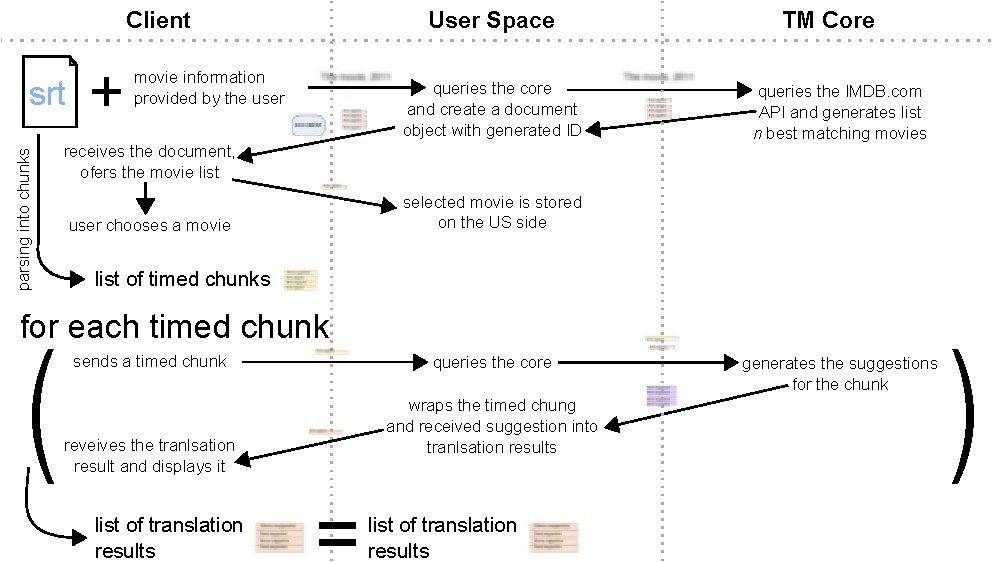
\includegraphics{figures/creating_document.pdf}
\end{center}
\caption{Structure of component communication during a new document creation}
\end{figure}

When a new document is created, the User Space receives basic information about the movie or TV show first. Based on that, it creates a Document object and saves it to the database immediately to receive a unique database ID which is then used as a document identifier in all the following calls. The core is called at this moment to provide a list of possible movies with matching title and year of production together with genre tags obtained from the Freebase knowledge base. The user is then supposed to choose one or none of the suggested movies. This information is used by the User Space at the moment the Core is queried for the translation suggestions.

When a new document is created, the client application sends a list of all chunks that the document consists of, and the User Space adds these chunks to the appropriate document.
Then, the client application starts to send batches of chunks to be translated. When the User Space receives such a call, it queries the TM Core for the translation suggestions.
Once the suggestions are generated, they are sent to the GUI; they do not persist in the User Space in any way. One reason to possibly keep the suggestions in memory or in the database would be to avoid regenerating them. However, we decided that the cost of regenerating the suggestions is smaller than the cost of additionally storing suggestions in memory or in the database, which would increase the memory requirement significantly. When the client queries saved translation results, they will be sent without translation suggestions. For each untranslated chunk in the document, suggestions are generated and sent to the GUI on demand (see the GUI documentation in Section~\ref{sec:document_translation}).

User Space also provides feedback to the translation memory. A list of new translations the users have produced can be generated together with information on which translation pair they used for post-editing. This information is provided to the Data Import module which adds the new translations to the translation memory and also uses the data for training the scoring of the suggestions (see Section~\ref{sec:ranking} in the Core documentation).

Export of the subtitle files is also solved in the User Space. It is described in more detail in Section~\ref{sec:export}.

\section{User Management}
\label{us:usermanag}
Because our own experience was that requiring a registration from a web service often prevented us from using it, we decided to make the registration as easy as possible. We have no constraints on user names (except for non-emptiness) and very little constraints on password (only it must be at least 3 characters long).

%KB: I don't like this
%We think the most important feature of a password is for the user to remember it, so w

We leave the assessment of the strength to the user. The password strength constraints are often rather arbitrary and many classes of strong passwords do not pass them, it is hard to develop a reasonable strength measure. 

%KB: these are paragraphs about nothing (sorry)
%E.g.\ a whole sentence, a "passphrase", is a very strong password; however, it usually does not pass measures requiring use of specific classes of characters. And vice versa, a password using very unusual characters (e.g.\ Czech letters with diacritic signs) can be impossible to break even if it is quite short, because the attacker simply does not try out such characters that are uncommon in passwords; still it often does not pass typical minimum password length constraints.

%Moreover, we are not forced to pay much attention to the security of the application - it does not contain any sensitive data whose compromising would pose a threat to the users of the application and the benefit to the attacker successfully breaking into a user account is close to none.

We allow the user to work in multiple browser tabs or windows, provided it is the same session (i.e.\ it has the same {\tt SessionID}), because we believe it is natural to work on multiple translations at once, to have the Document List opened to see the translation progress, etc. The user himself is responsible for having the same document opened multiple times, which is not expected behavior and so changes to the document in one Translation Workspace are not projected into the other Workspace until reloaded.

However, we decided to disallow one user having multiple sessions at one time, since it would cause problems to us when implementing it and it doesn't happen very often in our opinion. We do not support multiple users collaborating on one subtitle file at the moment.

As described in \ref{us:openid}, if a user registers through OpenID, we have to assign a user name to him (the unique OpenID identifier we get is typically a long hash, which does not look like a nice user name), see Section~\ref{subsubsec:gui_openid}. Because the user name is at least partly generated, the user might not like it. Therefore, we offer each user the possibility to change the user name (provided that the one he chooses is free). The user name is only used to authenticate the user (if not using OpenID login) and is displayed in the top right corner in the application; the internal unique identifier of a user is his user id, an integer assigned to each user on registration that never changes.

\section{Implementation Details}
\subsection{Data Types Overview}

The User Space uses the shared classes used throughout the application, or wrappers of such classes. A brief overview of the classes used and their roles in the User Space follows. We use the abbreviation US to refer to the User Space in the following sections.

\begin{itemize}
\item {\tt FilmtitBackendServer}  -- The class is the Java Servlet whose public methods are invoked by the RPC calls. Its main task is to mediate the calls to concrete opened sessions and take care of users login. A thread checking if there is a session without activity for a long time and terminating the non-active sessions is run in the server class.

\item {\tt Session} -- The class represents a running session and processes the client calls. There is exactly one session object for one logged in user. It contains hash tables of documents being currently edited to make them quickly accessible based on their IDs. During the existence of a session object, all the client-side operations are stored in memory and saved immediately to the database. When the session ends -- either by the user logging out or by exceeding the maximum time without a user action -- a record about the session is stored to database (ID of the user that owned the session, its start time and end time). This is intended as an activity log from which further statistics can be inferred.

\item {\tt USUser} -- This class is a wrapper of the shared User class. During the existence of the session, it is used as a provider of the documents owned by the user. It is also used for storing the settings of the user.

\item {\tt USDocument} -- The class is a wrapper of the shared {\tt Document} class. A {\tt USDocument} object represents a subtitle file with additional information about the movie it belongs to. Its content is supposed to be a mirror image of the Document object on the client side. It contains a list of Translation Results representing the actual subtitle chunks if the document is loaded to be edited. It is not connected to the translation results by the database mapping to make it easy to send a list of the user's documents without the actual content.

\item {\tt USTranslationResult} -- This class is a wrapper for the shared {\tt TranlsationResult} class. The class congregates the original subtitle chunk, its timing, the translations suggested by the translation memory, and the results of the user activity -- the users' translations and information about which translation suggestion they chose. It is the class where the actual translation is performed. Although a user can delete the document, all the translation results are kept in the database to provide feedback to the translation memory.

\item {\tt Emailer} -- A class used for sending email from the application. It is used for confirmation of user registration and also when the user forgets his password and requires sending a new one via email.

\end{itemize}

There are also two third-party classes included in the User Space source code. It is the {\tt IdGenerator} class which generates session IDs (distributed under the {\it Apache License, Version 2.0}) and the {\tt BCrypt} class which ensures hashing the passwords before we store them in the database (distributed under {\it BSD licence}).

The {\tt SubtitleDownloadServlet} class responsible for exporting the subtitle files is described in Section~\ref{sec:export}. Details concerning the user registration, login and using open ID are discussed in more detail is Section~\ref{subsec:simple_login} in the GUI chapter. Details about handling the communication with the client are covered in Section~\ref{sec:communication} of the GUI chapter.

\subsection{Database Mapping}
\label{subsec:database_mapping}

As mentioned before, the User Space mirrors all the client's operations and makes them persistent on the server side. The persistence is ensured by saving the data to the database. There are a number of sophisticated tools for the JVM to ensure data persistence, e.g.\ the \emph{Java Persistence API} framework, or some frameworks working on a higher level of abstraction, such as \emph{Spring Data Framework}. Since only very basic database operations are required during the operation of the User Space -- loading and saving of the raw Java objects -- only an object relational mapping library is used, namely \emph{Hibernate}. The structure of the database being mapped is displayed in Figure~\ref{fig:em_of_us}.

The mapping reflects the data properties of classes. If the class is a wrapper of a shared class, the getters and setters of the properties are bound to the wrapped objects properties.

As mentioned before, the mapping of {\tt USDocument} does not include the list of Translation Results the document contains in order to be able to send the documents both with and without the translation results. It would also be possible to use lazy Hibernate collection mappings, but it would cause problems at the time the object are serialized.

\begin{figure}
\begin{center}
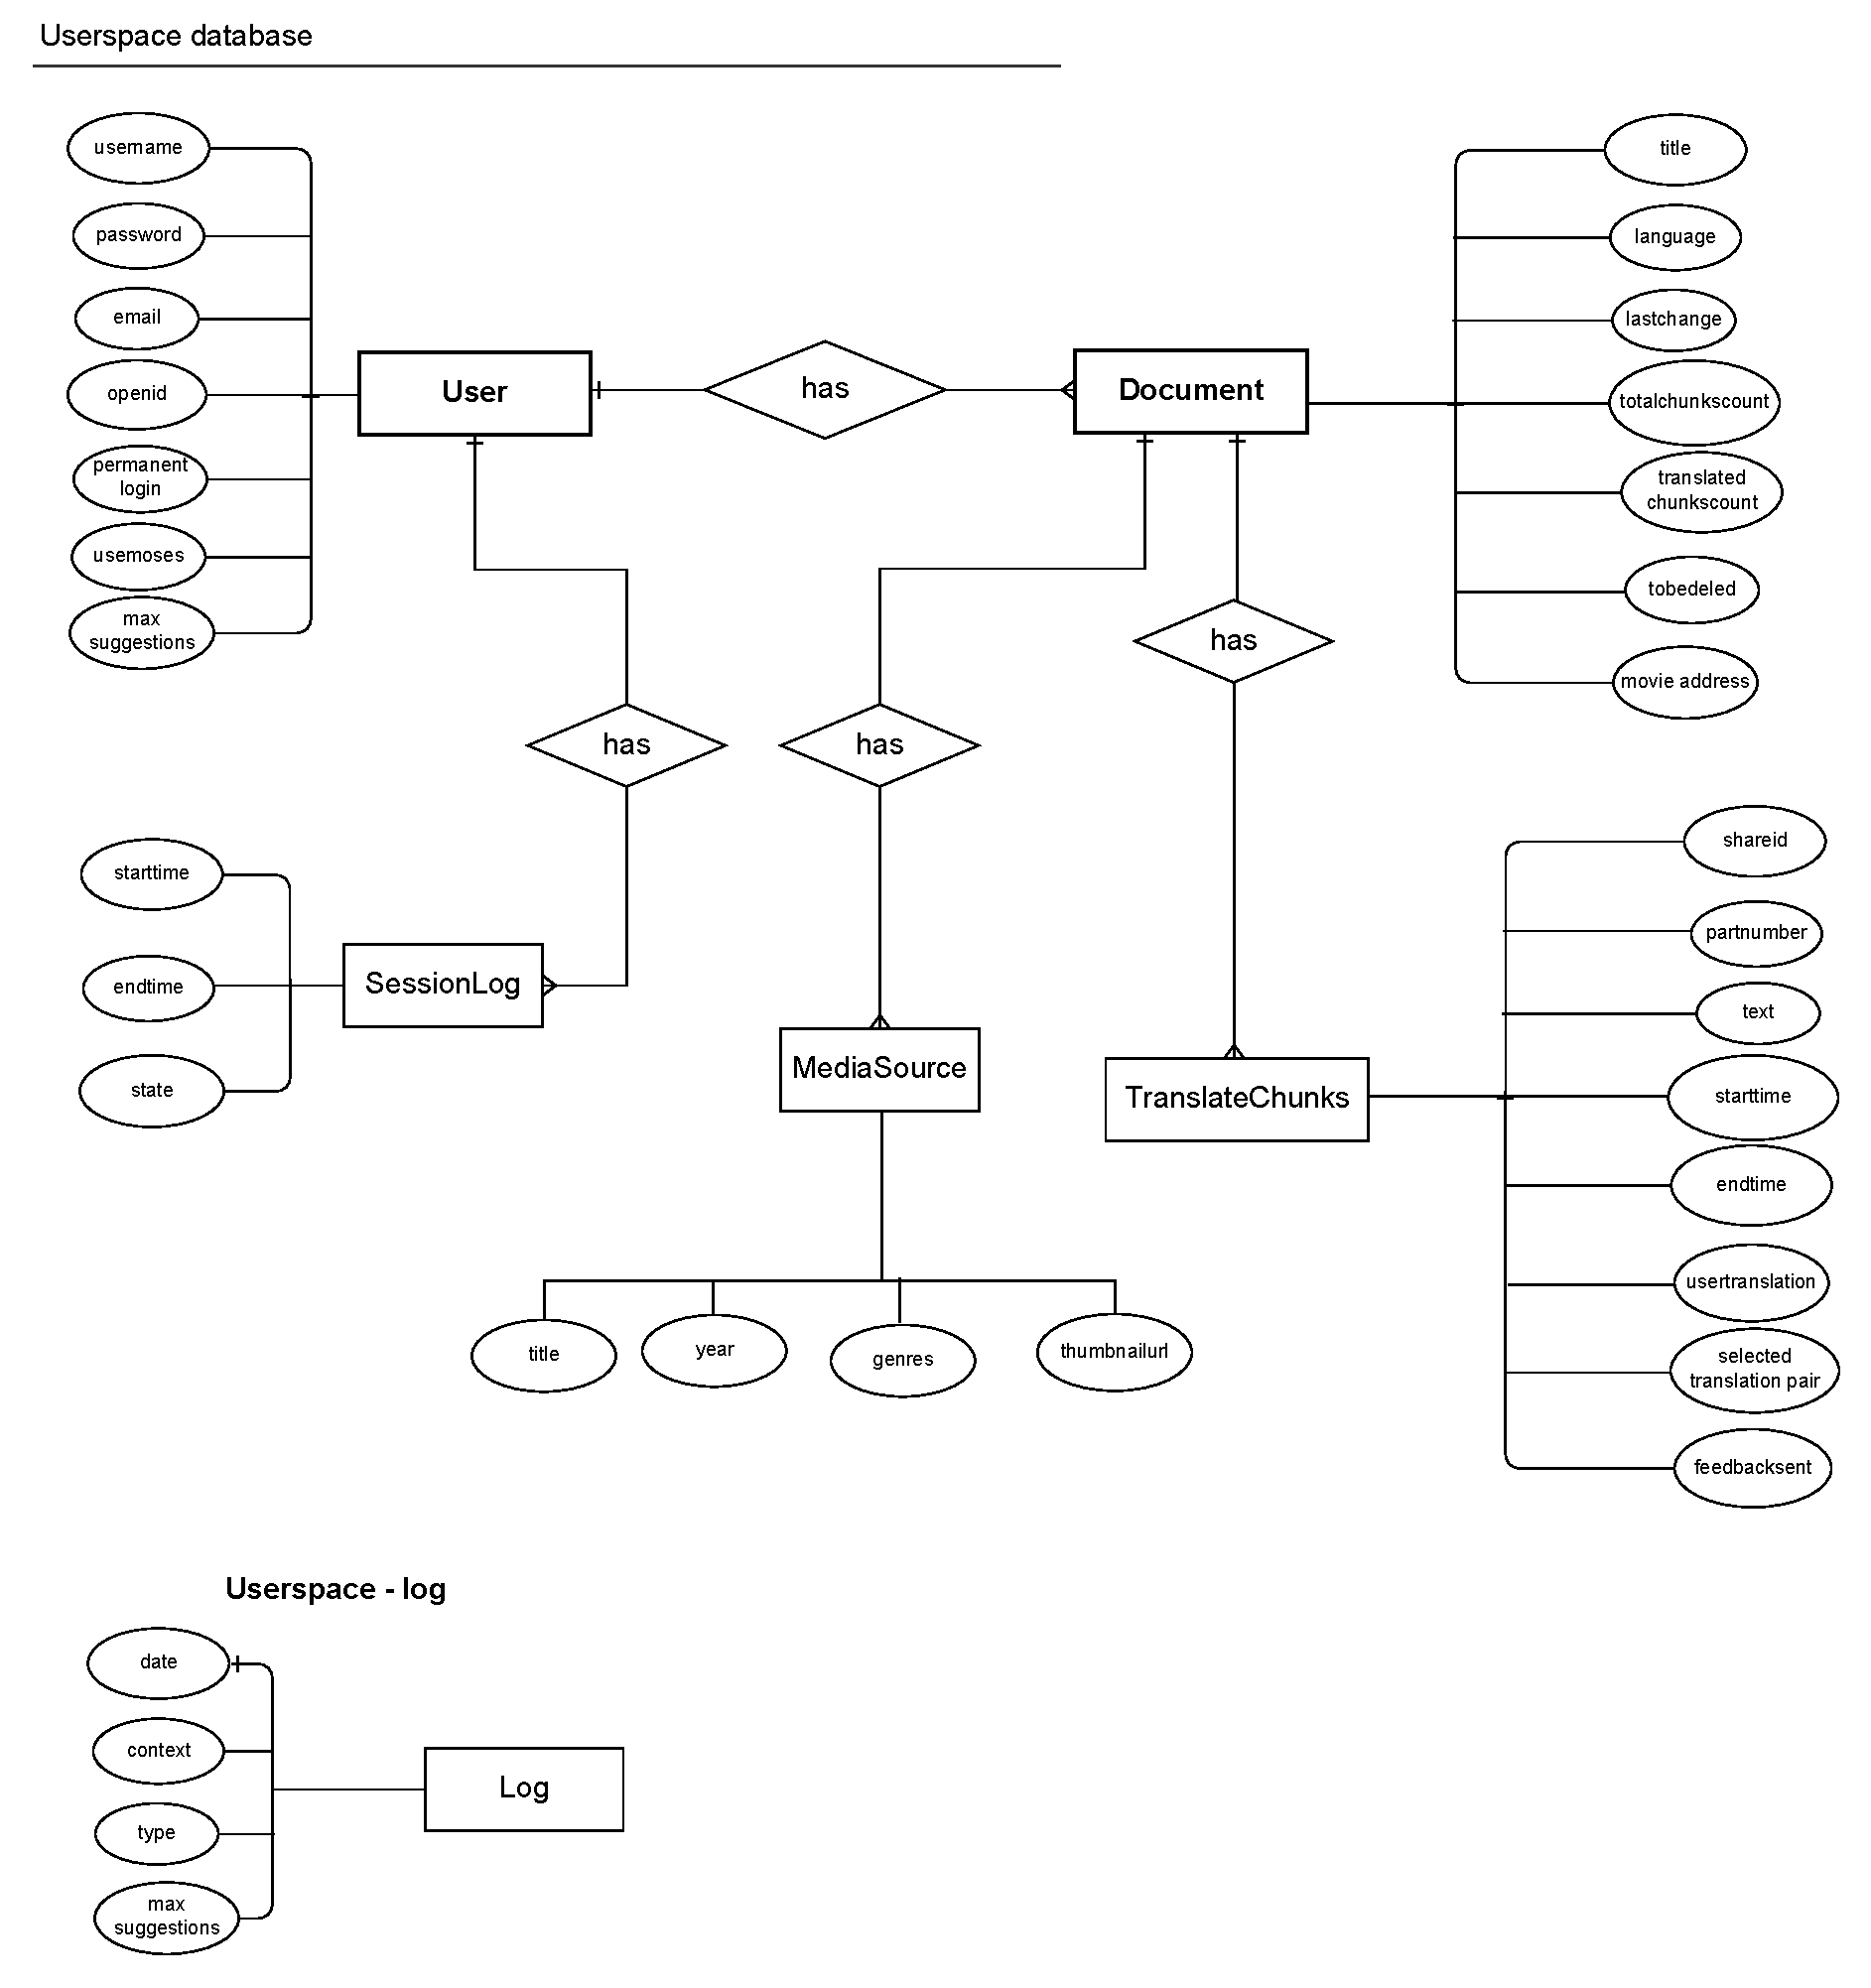
\includegraphics[scale=0.5]{figures/userspacedb.pdf}
\end{center}
\caption{EM diagram of the database used by the User Space}
\label{fig:em_of_us}
\end{figure}

\subsection{Providing Feedback to the Translation Memory}

In order to be able to provide feedback to the translation memory and take advantage of the translator work for improving the translation memory, the implementation of deleting a document and the selection of the media source should not be done synchronously. Handling this requirements is described in following paragraphs.

The User Space and the Translation Memory Core use the same database table for media sources (representing the movie or the TV show the subtitles are from). When the users create a document, they are required to enter the title of the movie about to be translated. After that, the {\it Freebase} service is queried for the movies and TV shows possibly having such title and a list of these matches is provided to the user to choose from. After the user chooses the media source, the media source object is sent back to the User Space. Then, a search in the database table for media sources is performed. If there is a record with the same title and the release year, its data (genres and thumbnails URL) are updated, if it is a completely new media source, it is saved to the table.

The reason for doing this is not to have duplicate media sources in the database and also the fact that the meta data of the movie should be available to the Data Import module when the feedback to the translation memory is provided.

Another issue to be mentioned here is the handling of document deletion. When the user clicks on the delete button in the interface, the document is marked to be deleted in the User Space and is removed from the list of documents owned by the user and from the list of documents that has been loaded during a session. From that time the document is not available to the user. A thread is then run that deals with the translation results the document consists of. All the translation results that have already been used as feedback to the translation memory are deleted from the database. If the document is empty after this step, it is deleted too.

Providing the feedback itself is done by a static method of the {\tt USTranslationResult} class. This method returns all the translation results what have not been used for feedback yet ({\tt hasSentFeedback} flag set to false). The translation results are provided with a reference to a document they belong to which allows to resolve the media source later. If the translation results come from a document that has been flagged as ready to be deleted, both the translation results and the document are deleted. Otherwise, the flag informing about having provided the feedback is set.

\subsection{OpenID}
\label{us:openid}
Apart from normal login, we also use OpenID for registration and login.

OpenID\footnote{\url{http://openid.net/}} is ``an open standard that describes how users can be authenticated in a decentralized manner, eliminating the need for services to provide their own ad hoc systems and allowing users to consolidate their digital identities'' (from Wikipedia).\footnote{\url{http://en.wikipedia.org/wiki/OpenID}}

We use \emph{JOpenID} for OpenID authentication. The positive aspect of \emph{JOpenID} is that it is easy to implement and use; the negative aspect is that it does not support arbitrary OpenID URLs, so we (as the web application developers) have to list the OpenID providers that we decide to support and let the user to choose only from these. From JOpenID documentation:\footnote{\url{http://code.google.com/p/jopenid/wiki/FAQ}}

\begin{quote}Yes OpenID standards contains two parts: \textbf{discovery} and \textbf{authentication}. Discovery is the process where the RP uses email or URL to look up the address of OP. It is complex, and may confuse the end users.

Instead, Web UI designer should give end users the chooses of their familiar OpenID accounts, such as Google account, Yahoo account, etc.

JOpenID only supports OpenID authentication because the discovery protocol is hard to use, and difficult to implement. You will find that JOpenID meets your 99.9\% requirements.
\end{quote}

We support Google, Yahoo and Seznam.cz;\footnote{\url{http://seznam.cz}, a Czech web portal, one of the largest Czech OpenID providers} this is done by implementing {\tt{cz.filmtit.userspace.login.SeznamData}}. We think that just a very small percentage of users actually know what OpenID is; therefore, allowing to login via Google, Yahoo and Seznam accounts seems sufficient.

However, there is a question to solve -- what to do when the user logs in through OpenID for the first time, because the user still needs to be in our database as a regular user. We were thinking about requiring an explicit registration, but that is unneccessary and complicated. Therefore, we register the OpenID user transparently.

Because we register the users as full users, we generate a username and password for them and then send these to their e-mail addresses, which  can be acquired from the OpenID provider. The users can thus log in even without their OpenID; they also have the possibility to change their username and/or password on the Settings page.


\section{Exporting Subtitle Files}
\label{sec:export}

Users can export the files in {\tt .srt} format. We decided to ignore the {\tt .sub} format because, as is shown in \ref{sec:properties}, in the initial data, the percentage of usage for {\tt .sub} was minimal and the work needed would be too big.

Exporting the files is a straightforward task -- we traverse the chunks, connect them to subtitle items if they have the same time, and save their contents.

%However, there is a problem with the formats. While .srt format uses time information, .sub format uses frames. For transfering between them, you have to know the FPS (frames per second) of the actual movie file. FPS varies across files (it is usually between 23 and 50, depending on the source of the movie file).

%Right now, we ask the user for FPS when exporting. Another solution would be to read the FPS from video file, loaded through the player (more about the player in ???), since VLC plug-in can read the FPS using javascript; we didn't implement that due to time constraints.

The issue with exporting is that we want to make the {\tt .srt} file downloadable. This cannot be done using only GWT and RPC, since GWT works through Javascript, which cannot produce files for download. So instead, we run a separate servlet, whose only responsibility is to produce {\tt .srt} files. This servlet, named \texttt{SubtitleDownloadServlet}, is created at the start of the program, has a \texttt{FilmTitBackendServer} reference, and receives document ID, session ID and the file type through a standard GET request. First, it is checked if the session ID is correct, then if the users own the given document, and if they do, a file is created. Sequence diagram of  dowloading the exported subtitles is in Figure~\ref{fig:export_diagram}

\begin{figure}[h]
\begin{center}
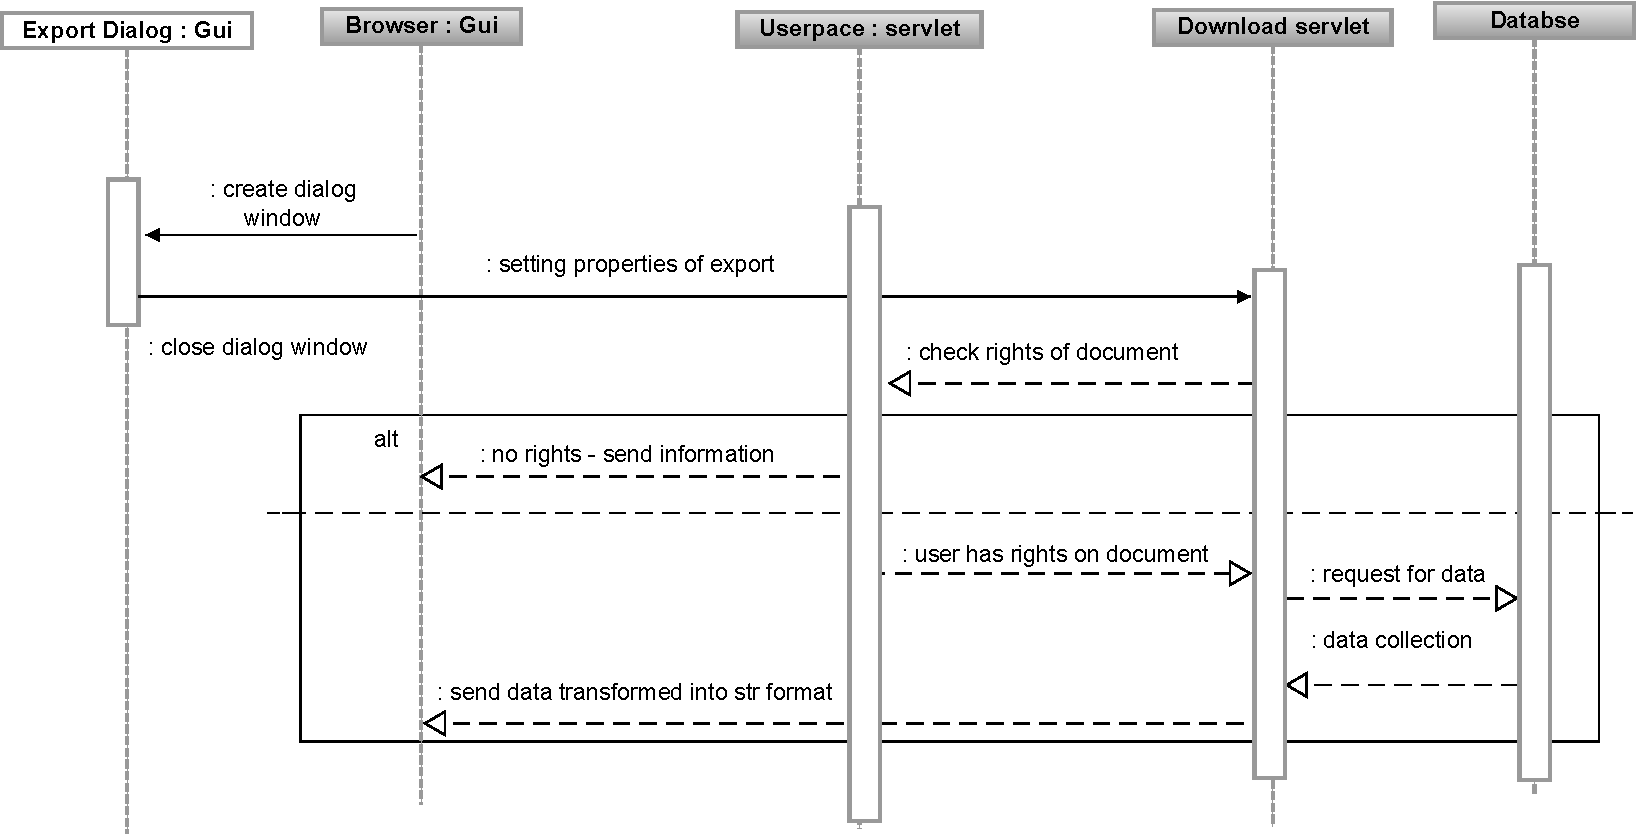
\includegraphics[scale=0.6]{figures/download_diagram.pdf}
\end{center}
\caption{Sequence diagram of exporting a subtitle file}
\label{fig:export_diagram}
\end{figure}

We can export three different types of file:
\begin{itemize}
    \item a file with only the translated chunks, completely omitting the untranslated ones,
    \item a file with the translated chunks, with the source chunks at places where nothing is translated,
    \item a file with only the source chunks.
\end{itemize}

All three types are either in {\tt .srt} or {\tt .txt} format. The {\tt .txt} format is just the text of the subtitles without any time information.